\documentclass[11pt,border=4pt]{standalone}
\usepackage{amsmath,amssymb,bm,mathtools}
\usepackage[fontset=fandol]{ctex}
\usepackage{tikz}
\usetikzlibrary{arrows.meta,calc,patterns,angles,quotes,decorations.markings,decorations.pathmorphing}
\newcommand{\dd}{\mathop{}\!\mathrm d}
\newcommand{\e}{\mathrm e}
\tikzset{axis/.style={->,>=Stealth,line width=.45pt},world/.style={line width=.8pt},flow/.style={->,>=Stealth,line width=.7pt},ray/.style={->,>=Stealth,line width=.7pt},guide/.style={dashed,line width=.35pt},aux/.style={dashed,line width=.35pt},dim/.style={<->,>=Stealth,line width=.35pt},every node/.style={font=\small},force/.style={->,>=Stealth,very thick},gas/.style={fill=blue!7}}
\begin{document}
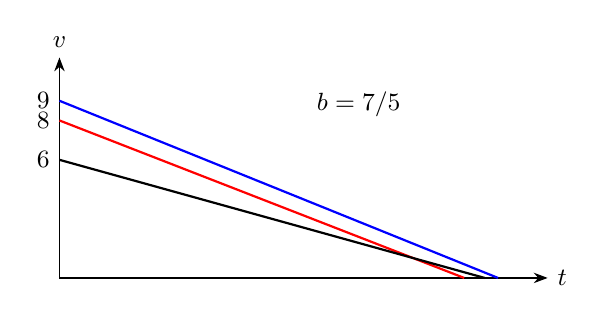
\begin{tikzpicture}\draw[axis](0,0)--(6.2,0)node[right]{$t$};\draw[axis](0,0)--(0,2.8)node[above]{$v$};\draw[world,blue](0,2.25)--(5.57,0);\draw[world,red](0,2)--(5.14,0);\draw[world](0,1.5)--(5.4,0);\node[left]at(0,2.25){$9$};\node[left]at(0,2){$8$};\node[left]at(0,1.5){$6$};\node at(3.8,2.2){$b=7/5$};\end{tikzpicture}
\end{document}
